\documentclass[11pt,a4paper]{article}

\usepackage[margin=2.4cm]{geometry}
\usepackage{amsmath,amssymb}
\usepackage{booktabs}
\usepackage{graphicx}
\usepackage[table]{xcolor}
\usepackage{caption}
\usepackage[hidelinks]{hyperref}
\usepackage{natbib}
\usepackage{microtype}

\captionsetup{font=small,labelfont=bf}
\setlength{\parskip}{0.35em}
\bibliographystyle{apalike}

\title{\bf Cost-aware deep allocation across published asset-pricing anomalies}
\author{Alban Br\'eart de Boisanger\\[2pt]
\small Machine Learning in Finance (FIN-407), EPFL}
\date{}

\begin{document}
\maketitle

\begin{abstract}
\noindent
We ask what is gained by training a neural network on the objective a fund is
actually paid for --- the Sharpe ratio of a book net of trading costs --- rather
than on squared forecast error. The asset universe is the 212 published
cross-sectional anomalies of the Open Source Asset Pricing project, assembled
point-in-time by publication date; the problem is how much capital to allocate to
each, monthly. One permutation-equivariant architecture is trained under four
objectives with data, folds and portfolio construction held fixed. Over 203
out-of-sample months (2008--2024) the ranking of models by gross Sharpe ratio and
by net Sharpe ratio differs sharply: all nine models look comparable gross
(0.94--1.38), but net of measured anomaly-specific costs only the two cost-aware
objectives clear the equal-weighted benchmark, and five lose money outright. The
model with the \emph{highest} information coefficient earns a net Sharpe ratio of
0.19; the model with the \emph{lowest} earns 0.45. No model beats $1/N$
significantly, but the cost-blind ones lose to it significantly. We show the
mechanism is not the expected one --- the cost-aware model does not avoid
expensive anomalies, it stops rebalancing.
\end{abstract}

\section{Introduction and problem statement}

A machine-learning pipeline for asset returns usually minimises a pointwise loss
and then, separately, sorts the resulting forecasts into a portfolio. The two
steps optimise different things. Squared error weights an observation by its
return variance rather than by the capital that can be deployed against it; it is
indifferent to the cross-sectional ordering, which is what a portfolio actually
monetises; and it knows nothing about turnover, so two models with identical
forecast accuracy --- one producing stable rankings, one reshuffling every month
--- are treated as equally good and are worth very different amounts of money.

Portfolio construction, however, is differentiable. Mapping scores to weights is a
demeaning and a normalisation; turnover is an $L_1$ distance to last month's
drifted book. The entire path from features to net-of-cost profit can therefore be
back-propagated through, and the network can be asked to maximise the quantity the
fund is paid for. This paper measures what that is worth.

We deliberately study the problem one level above stock selection. The assets are
the published anomalies themselves, so the allocation decision is the one a
multi-strategy fund faces: given a menu of documented, replicated strategies, each
with its own return, risk and \emph{cost of being held}, how should capital be
spread across them? This setting has a property that makes the cost question
sharp. The intrinsic turnover of an anomaly's underlying stock book varies by a
factor of 500 --- an annual-accounting signal barely moves, an
analyst-revision signal is rewritten every month --- so the cost of \emph{holding}
a sleeve differs enormously across the menu, quite apart from the cost of changing
one's mind about it.

Three hypotheses are tested, each isolating one change: whether seeing the whole
cross-section helps (\S\ref{sec:models}), whether optimising the ordering beats
optimising the level, and whether optimising net-of-cost profit beats optimising
the ordering.

\section{Data and feature engineering}

\paragraph{Returns.} The long-short monthly return of each of 212 predictors comes
from \texttt{PredictorPortsFull} in the Open Source Asset Pricing release
\citep{ChenZimmermann2022}. These are the assets we allocate across. Returns are
reported in percent and are converted to decimals; the portfolios are
equal-weighted decile spreads, self-financing, so no risk-free adjustment applies.

\paragraph{A point-in-time universe.} An anomaly enters the investable universe in
the January \emph{after} the year its paper appeared. An investor in 1980 could
not allocate to an anomaly documented in 2005, and a backtest that permits it is
measuring a time machine rather than a strategy. The screen is expensive: it cuts
173{,}302 anomaly-months to 50{,}370 and moves the sample start to 1994, because
fewer than 20 anomalies had been published before then. The universe grows from 22
assets in 1994 to 208 by 2020, which is itself an honest picture of what an
allocator's menu looked like through time. This construction also makes ``years
since publication'' a legitimate feature rather than a leak, since by construction
it is never negative.

\paragraph{Features.} Twenty-eight continuous features are built from information
dated $t$ or earlier: trailing cumulative returns over 1, 3, 6, 12, 24, 36 and 60
months (including the 12-month-skipping-one construction), realised volatility and
trailing Sharpe ratios, 60-month drawdown, skewness, and the anomaly's beta and
correlation to the equal-weighted index of all currently available anomalies.
Twenty-one indicators capture the strategy's own definition --- economic category,
data source, discrete versus continuous form, value versus equal weighting --- and
nineteen missingness flags mark where a feature could not be computed. Continuous
features are ranked within each month and rescaled to $[-1,1]$; indicators are left
alone, since ranking a binary column produces a number whose value depends on how
many peers share the category. Every transform is cross-sectional \emph{within a
month}, so no test-period distribution can leak into a training-period feature.

Variables that exist in the metadata but are not knowable at time $t$ are
excluded, even though they predict returns well: \citeauthor{ChenZimmermann2022}'s
replication-quality grades and the 2025 citation counts are assessments made in
the 2020s. Raw publication years are also dropped --- with only 212 assets they
come close to naming each anomaly, and a network given them can memorise which
specific anomalies paid off instead of learning what \emph{kind} of anomaly pays.

\paragraph{Costs, measured rather than assumed.} Allocating across anomalies
incurs two distinct costs. \emph{Switching} is paid on the change in allocation
weight. \emph{Carrying} is paid on the weight held, because the sleeve rebalances
its own stock book every month whether or not the allocator touches it. The second
is not published, but it is recoverable: the release also distributes the
firm-level signal behind each portfolio, so we rebuild each anomaly's decile book
month by month and measure how much of it turns over. Table~\ref{tab:turnover}
gives the range.

\begin{table}[t]
\centering\small
\caption{Measured monthly turnover of the underlying stock book, and the implied
cost of carrying the sleeve for a year at a 25\,bp one-way stock trading cost.}
\label{tab:turnover}
\begin{tabular}{lrr}
\toprule
& Monthly turnover & Carrying cost \\
\midrule
\texttt{CitationsRD}, \texttt{GP}, \texttt{PatentsRD} (annual accounting) & 0.008 & 0.02\,\%/yr \\
Median anomaly & 0.129 & 0.39\,\%/yr \\
\texttt{dCPVolSpread}, \texttt{ChangeInRecommendation} (options, analyst revisions) & 3.98 & 12\,\%/yr \\
\bottomrule
\end{tabular}
\end{table}

The estimate is used causally: at month $t$ the model and the cost model see an
expanding-window average of turnover realised strictly before $t$. This costs
nothing in accuracy, because turnover is close to a structural constant of each
signal --- its cross-decade correlation is between 0.985 and 0.997, since it is
determined by the sampling frequency of the underlying data. Anomalies documented
with multi-month holding periods roll only part of the book each month, so their
measured churn is divided by the holding period.

\section{Models}\label{sec:models}

\paragraph{Benchmarks.} The classical ladder --- Huber-loss OLS, ridge, elastic
net, partial least squares and gradient-boosted trees --- is fitted pooled, with
each hyper-parameter chosen on the fold's own validation block. The
\textbf{equal-weighted ($1/N$) allocation} is treated as a model and appears as a
row in every table, costed identically. It is famously hard to beat
\citep{DeMiguel2009}, and burying it in the text is how that fact gets hidden.

\paragraph{Networks.} \texttt{AssetMLP} is the \citet{GuKellyXiu2020} benchmark: a
feed-forward network applied to each asset-month independently, which cannot see
the rest of the cross-section. \texttt{CrossSectionalNet} is a Set Transformer
\citep{Lee2019}: assets exchange information through 32 learned inducing points,
costing $O(Nm)$ rather than the $O(N^2)$ of full self-attention. It is
permutation-equivariant by construction --- relabelling the assets permutes the
outputs identically --- so it can only learn from an asset's characteristics and
its peers' distribution, never from its position in the input. This is verified
numerically in the test suite to $3.6\times10^{-7}$. At 19{,}457 parameters it is
deliberately small; the panel has 48{,}236 rows.

\paragraph{Allocation.} Scores become weights as $1/N$ plus a dollar-neutral tilt
of fixed $L_1$ size. The benchmark an allocator must beat is equal weighting, so
the network is asked for the deviation from it; this also conditions training
well, since at initialisation the scores are noise and the portfolio starts life
as the benchmark rather than as a random book. A per-anomaly cap of 10\% is
enforced by fixing capped names and redistributing only across free ones, and the
book is scaled to a 10\% ex-ante volatility target using a strictly lagged
trailing estimate.

\paragraph{Objectives.} With weights $w_t$ set at the close of month $t$ and
earning $r_{t+1}$,
\begin{align}
\tilde w_{t-1} &= \frac{w_{t-1}\odot(1+r_t)}{1 + w_{t-1}^\top r_t},
&\text{(drifted book)}\\
c_t &= \textstyle\sum_i s_i\,\lvert w_{t,i}-\tilde w_{t-1,i}\rvert
      + \sum_i k_i\,\lvert w_{t,i}\rvert,
&\text{(switching + carrying)}\\
\mathcal{L}_{\text{Sharpe}} &= -\sqrt{12}\;
\frac{\overline{(w^\top r - c)}}{\mathrm{sd}(w^\top r - c)} .
\end{align}
Charging against the \emph{drifted} book matters: an allocation left untouched
still changes as sleeves earn different returns, and billing that as a trade
invents turnover that never happened. The mean--variance variant replaces the
Sharpe ratio with $\bar{x}-\tfrac{\gamma}{2}\mathrm{var}(x)$, which has the same
optimum at a given risk level but a far better-conditioned gradient when the
window is short. Two cost-blind objectives --- masked squared error and the
cross-sectional rank correlation --- are trained on the identical architecture, and
each model is early-stopped on \emph{its own} validation objective, so no model
borrows another's advantage.

\section{Evaluation methodology}

The sample is walked forward one year at a time. Each refit trains on everything
available up to a four-year validation block used for early stopping and
hyper-parameter selection, then predicts the following year, which it has never
seen. A \textbf{12-month embargo} separates training from validation, because
several anomalies are built from annual accounting data and a shorter gap would
place the same fundamentals on both sides of the boundary \citep{LopezDePrado2018}.
Seventeen folds produce 38{,}539 out-of-sample predictions per model, covering
2008-02 to 2024-12 without overlap; the test suite asserts these properties
mechanically rather than trusting the implementation. Neural results are averaged
over five seeds, since a single network fitted to monthly returns is a
high-variance estimator.

We report statistical and economic metrics separately because they can disagree,
and here they do. Out-of-sample $R^2$ follows \citet{GuKellyXiu2020} in
benchmarking against a zero forecast rather than the historical mean. Sharpe
ratios carry \citet{Lo2002} standard errors and Newey--West $t$-statistics. The
\emph{break-even cost} --- the one-way cost at which a strategy stops making money
--- is reported because it is assumption-free.

\section{Results}

\begin{table}[t]
\centering\small
\caption{Out-of-sample performance, 2008-02 to 2024-12 (203 months), net of
measured anomaly-specific costs. IC is the mean monthly rank information
coefficient. Break-even is the one-way stock trading cost at which the net return
reaches zero.}
\label{tab:main}
\begin{tabular}{llrrrrrr}
\toprule
Model & Objective & IC & Gross SR & \textbf{Net SR} & $t$ & Turnover & Break-even \\
\midrule
\texttt{xs\_utility}  & net-of-cost utility & 0.063 & 1.38 & \textbf{0.45} & 1.53 & 0.67 & 183\,bp \\
\texttt{xs\_sharpe}   & net-of-cost Sharpe  & 0.066 & 1.21 & \textbf{0.40} & 1.48 & 0.62 & 179\,bp \\
\rowcolor{black!7}
\texttt{equal\_weight}& \emph{$1/N$ benchmark} & --- & 1.32 & \textbf{0.39} & 1.44 & 0.09 & 866\,bp \\
\texttt{xs\_ic}       & rank correlation    & 0.101 & 1.17 & 0.19 & 0.82 & 0.91 & 115\,bp \\
\texttt{nn3\_mse}     & squared error, per-asset & 0.087 & 1.07 & 0.17 & 0.73 & 0.88 & 113\,bp \\
\texttt{gbrt}         & squared error, trees & 0.095 & 1.03 & $-0.01$ & $-0.03$ & 1.17 & 81\,bp \\
\texttt{xs\_mse}      & squared error       & 0.092 & 1.07 & $-0.02$ & $-0.08$ & 1.17 & 85\,bp \\
\texttt{pls}          & squared error, PLS  & 0.087 & 0.96 & $-0.03$ & $-0.15$ & 1.05 & 83\,bp \\
\texttt{ols\_h}       & Huber, linear       & 0.093 & 1.04 & $-0.07$ & $-0.29$ & 1.23 & 77\,bp \\
\texttt{ridge}        & squared error, linear & 0.086 & 0.97 & $-0.10$ & $-0.42$ & 1.17 & 75\,bp \\
\texttt{enet}         & squared error, sparse & 0.080 & 0.94 & $-0.30$ & $-1.21$ & 1.54 & 55\,bp \\
\bottomrule
\end{tabular}
\end{table}

\paragraph{Gross and net rank the models differently.} Table~\ref{tab:main} is the
paper's main result. Gross Sharpe ratios span 0.94--1.38 and every model is
broadly comparable; a study that stopped there would report nine successes. Net of
costs, only the two cost-aware objectives clear the benchmark and five models lose
money outright. The spread between best and worst net Sharpe ratio is 0.75, of
which almost none is visible gross.

\paragraph{Predictive accuracy does not order the models by economic value.}
\texttt{xs\_ic} attains the highest information coefficient (0.101) and the highest
out-of-sample $R^2$ (1.48\%) of any model and earns a net Sharpe ratio of 0.19.
\texttt{xs\_utility} has the \emph{lowest} IC (0.063) and the best net Sharpe
ratio. The two extremes are therefore inverted --- but we resist the stronger
claim: across all ten models the Spearman correlation between IC and net Sharpe
ratio is only $-0.14$ ($p=0.70$, $n=10$), which is indistinguishable from zero.
The defensible statement is the weaker and still useful one: \textbf{knowing which
model forecasts best tells you nothing about which model earns most}. Improving
forecast accuracy and improving the traded objective are different problems, and a
model-selection procedure that ranks on IC is choosing close to at random.

\paragraph{The honest significance statement.} Regressed on the benchmark,
\texttt{xs\_utility} has an alpha of $+1.46\%$/yr with a HAC $t$ of 0.88 and a beta
of 1.21, so part of the raw gap is leverage rather than skill; its information
ratio is 0.31 and the $t$ on its active return is 1.15. \textbf{No model beats
$1/N$ at conventional significance.} What \emph{is} significant is the damage done
by the cost-blind objectives: \texttt{ridge} ($t=-1.97$), \texttt{xs\_mse}
($-2.08$) and \texttt{enet} ($-2.55$) destroy value against equal weighting. The
defensible claim is therefore not that machine learning beats naive
diversification; it is that the choice of objective decides whether ML allocation
loses to $1/N$ or merely ties it.

\begin{figure}[t]
\centering
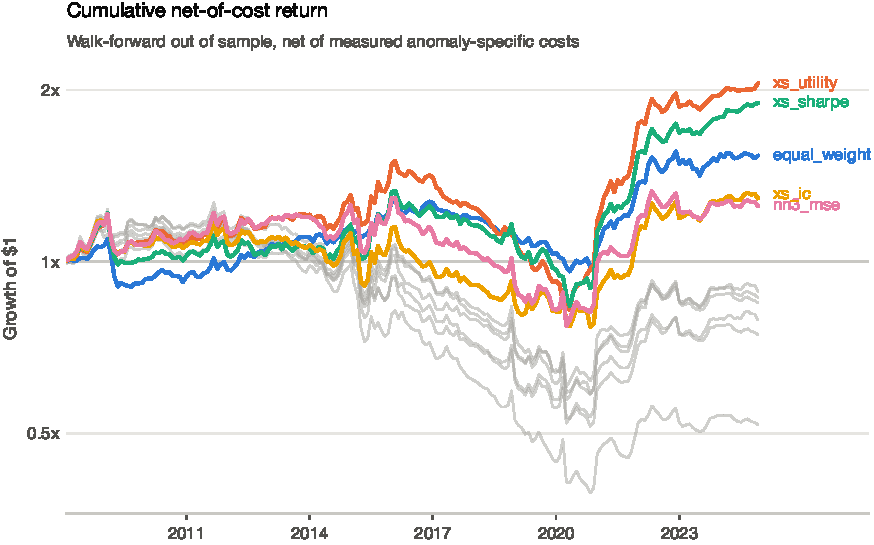
\includegraphics[width=\textwidth]{figures/f1_cumulative.pdf}
\caption{Cumulative net-of-cost return, walk-forward out of sample. Grey lines are
the seven models not named.}
\label{fig:cum}
\end{figure}

\paragraph{The mechanism is not the expected one.} The natural hypothesis is that
a cost-aware model learns to avoid anomalies that are expensive to carry. It does
not. Sorting anomalies into quintiles by measured carrying cost, the best model's
average tilt away from $1/N$ is $-0.0007$ on the cheapest quintile and $+0.0004$ on
the dearest --- flat, and if anything mildly the wrong way. What it learns is
\emph{allocation persistence}. Turnover falls from 0.88--1.54 to 0.62--0.67 and the
annual switching bill from 5.3--9.2\% to 3.7--4.0\%, while carrying cost is similar
for every model (3.9--6.1\%) because all of them end up holding close to the full
menu. Figure~\ref{fig:decomp} shows the decomposition: the edge is in not
rebalancing, not in what is held.

\begin{figure}[t]
\centering
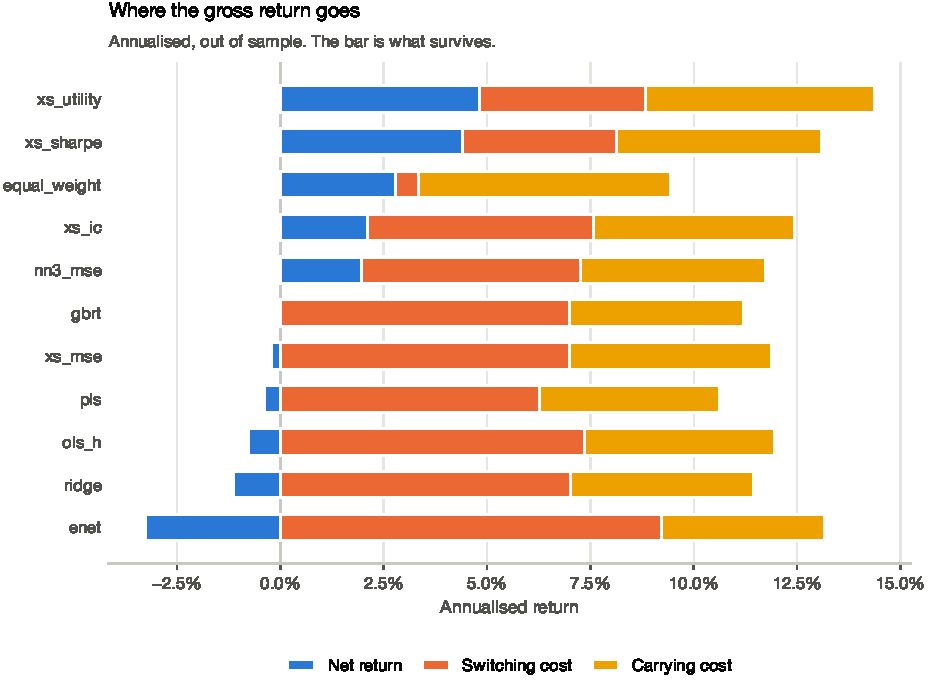
\includegraphics[width=\textwidth]{figures/f6_cost_decomposition.pdf}
\caption{Annualised gross return split into switching cost, carrying cost and what
survives.}
\label{fig:decomp}
\end{figure}

\paragraph{Robustness.} Figure~\ref{fig:cost} scales both cost components together.
At zero cost the models and the benchmark are nearly tied (1.32--1.38), confirming
that essentially all of the observed differentiation is a cost phenomenon. The
ordering in Table~\ref{tab:main} is stable across the whole grid, and the
cost-aware objectives degrade most slowly. Splitting the sample at 2015,
\texttt{xs\_utility} earns net Sharpe ratios of 0.47 and 0.45 in the two halves
while \texttt{enet} deteriorates from $0.00$ to $-0.44$; the cost-aware result is
not driven by one sub-period.

\begin{figure}[t]
\centering
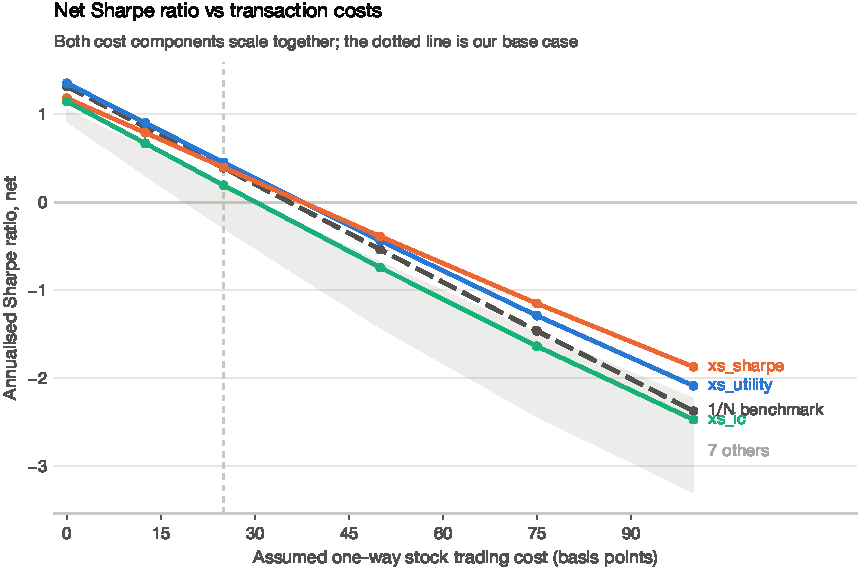
\includegraphics[width=\textwidth]{figures/f2_cost_sensitivity.pdf}
\caption{Net Sharpe ratio as both cost components are scaled. The dotted line is
the 25\,bp base case; the grey band spans the seven unnamed models.}
\label{fig:cost}
\end{figure}

\section{Capacity: does any of this survive in tradable stocks?}

Published anomaly returns are concentrated in small, illiquid names, so a result
obtained on the unrestricted universe may describe a portfolio no fund could run.
The release distributes every anomaly rebuilt using only stocks above the NYSE
20th percentile of market capitalisation; we repeat the entire study on that
universe, refitting every model on its own walk-forward folds.

The restriction is expensive before a single basis point of cost. The mean
long-short return falls from 0.499\% to 0.348\% per month, and at zero assumed
cost the benchmark's Sharpe ratio falls from 1.32 to 0.80 --- a 40\% haircut.
Table~\ref{tab:capacity} shows what is left after costs.

\begin{table}[t]
\centering\small
\caption{Net Sharpe ratio in both universes. The right-hand columns sweep the
assumed one-way stock trading cost; 12.5\,bp is arguably the right figure for a
large-capitalisation universe, and 25\,bp the right one for the unrestricted
sample.}
\label{tab:capacity}
\begin{tabular}{lrrrrr}
\toprule
& \multicolumn{2}{c}{All stocks} & & \multicolumn{2}{c}{Large caps only} \\
\cmidrule(lr){2-3}\cmidrule(lr){5-6}
Model & 12.5\,bp & 25\,bp & & 12.5\,bp & 25\,bp \\
\midrule
\texttt{xs\_utility}   & 0.90 & \textbf{0.45} & & 0.26 & $-0.25$ \\
\texttt{xs\_sharpe}    & 0.79 & 0.40 & & 0.20 & $-0.28$ \\
\rowcolor{black!7}
\texttt{equal\_weight} & 0.86 & 0.39 & & \textbf{0.34} & $-0.12$ \\
\texttt{xs\_ic}        & 0.67 & 0.19 & & 0.04 & $-0.59$ \\
\texttt{enet}          & 0.30 & $-0.30$ & & $-0.13$ & $-0.85$ \\
\bottomrule
\end{tabular}
\end{table}

Two things follow, and the second is the more important.

\paragraph{The ranking of objectives survives; the edge does not.} The rank
correlation of net Sharpe ratios across the two universes is $+0.75$: cost-aware
objectives still beat cost-blind ones, and \texttt{enet} is still last. The
paper's claim about \emph{objectives} is therefore not an artefact of an
untradable sample. But every point in Figure~\ref{fig:capacity} lies below the
45-degree line and every one is negative --- at 25\,bp, nothing in the tradable
universe makes money, benchmark included.

\paragraph{Where the model's advantage does survive, it reverses.} At 12.5\,bp,
a defensible cost for large capitalisations, the best allocation in the tradable
universe is \textbf{equal weighting} (0.34), ahead of \texttt{xs\_utility}
(0.26) and \texttt{xs\_sharpe} (0.20). The cost-aware models beat $1/N$ in the
universe where anomalies are strong and expensive, and lose to it in the universe
where they are weak and cheap. Read together with \S5, the honest summary of this
project is narrow: \emph{the choice of training objective reliably separates good
ML allocation from bad, and no version of it reliably beats doing nothing.}

\begin{figure}[t]
\centering
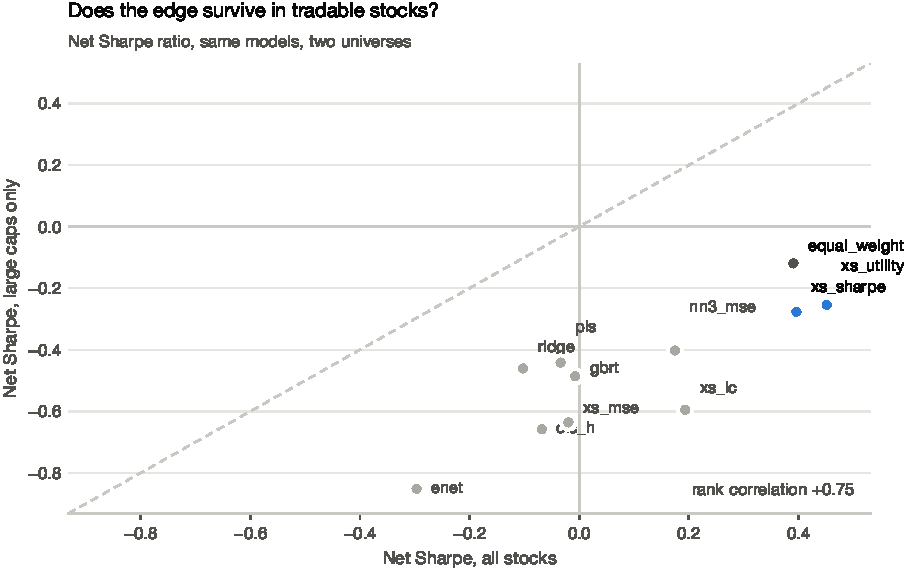
\includegraphics[width=0.92\textwidth]{figures/f9_capacity.pdf}
\caption{Net Sharpe ratio of the same models in both universes, at the 25\,bp
base case. Every model falls below the 45-degree line.}
\label{fig:capacity}
\end{figure}

\section{Conclusion and extensions}

Training a network on net-of-cost portfolio profit rather than on forecast error
changes an allocation that loses to equal weighting into one that ties it, and it
does so through a mechanism --- refusing to rebalance --- that a pointwise loss
cannot express. The negative half of this finding is the statistically solid half:
cost-blind machine learning applied to anomaly allocation destroys value against a
benchmark that requires no model at all.

Three extensions follow directly. First, the no-trade band: our allocator
rebalances every month by construction, whereas the natural response to a
turnover penalty is a hold region, and solving for it explicitly should widen the
gap this paper measures. Second, a lower-cost tradable universe: \S6 shows the large-cap
result hinges on the assumed spread, and a proper treatment would estimate the
spread per anomaly from the actual market capitalisations it holds rather than
applying one number to the whole universe. Third, sample length: 203 out-of-sample months cannot resolve a
0.06 difference in Sharpe ratio, and the point-in-time publication screen is what
costs us the earlier data --- relaxing it would be dishonest, but reporting the
hindsight-universe result alongside would bound how much the screen costs.

\paragraph{Code and reproducibility.} All data is free and public; \texttt{make
all} reproduces every number from a clean clone. The codebase is 20 modules with
52 tests, built around synthetic panels where the answer is known: the pipeline
must recover a planted signal and must find nothing in pure noise. Libraries used:
PyTorch, scikit-learn, LightGBM, Polars, pandas, NumPy, SciPy, statsmodels,
Matplotlib.

\begin{thebibliography}{9}\small
\bibitem[Chen and Zimmermann(2022)]{ChenZimmermann2022}
Chen, A. Y. and T. Zimmermann (2022). Open Source Cross-Sectional Asset Pricing.
\emph{Critical Finance Review} 27(2), 207--264.
\bibitem[DeMiguel et al.(2009)]{DeMiguel2009}
DeMiguel, V., L. Garlappi and R. Uppal (2009). Optimal Versus Naive
Diversification. \emph{Review of Financial Studies} 22(5), 1915--1953.
\bibitem[Gu et al.(2020)]{GuKellyXiu2020}
Gu, S., B. Kelly and D. Xiu (2020). Empirical Asset Pricing via Machine Learning.
\emph{Review of Financial Studies} 33(5), 2223--2273.
\bibitem[Lee et al.(2019)]{Lee2019}
Lee, J., Y. Lee, J. Kim, A. Kosiorek, S. Choi and Y. W. Teh (2019). Set
Transformer. \emph{ICML}.
\bibitem[Lo(2002)]{Lo2002}
Lo, A. (2002). The Statistics of Sharpe Ratios. \emph{Financial Analysts Journal}
58(4), 36--52.
\bibitem[L\'opez de Prado(2018)]{LopezDePrado2018}
L\'opez de Prado, M. (2018). \emph{Advances in Financial Machine Learning}. Wiley.
\bibitem[McLean and Pontiff(2016)]{McLeanPontiff2016}
McLean, R. D. and J. Pontiff (2016). Does Academic Research Destroy Stock Return
Predictability? \emph{Journal of Finance} 71(1), 5--32.
\bibitem[Novy-Marx and Velikov(2016)]{NovyMarxVelikov2016}
Novy-Marx, R. and M. Velikov (2016). A Taxonomy of Anomalies and Their Trading
Costs. \emph{Review of Financial Studies} 29(1), 104--147.
\end{thebibliography}

\end{document}
